\chapter{StARAPTOR: A Review-powered Tool for KPI Forecasting}
\label{chap:methodology}

\section{Research Questions}
\label{sec:research_questions}

Based on the objectives defined in Section \ref{sec:objectives} and on the exploration of the State of the Art conducted in Chapter \ref{chap:state_of_the_art}, three research questions have been defined and answered to ensure that the defined system represents an actual improvement to the state of the art.

\rqbox{1}{Is LLM-based NLP consistent enough to be used in analysis?}

\rqbox{2}{Is Association Mining a solid approach to find review patterns?}

\rqbox{3}{Is Time-Series Forecasting on Key Performance Indicators (KPIs), Preprocessed Reviews and Mined Associations an improvement on KPI-only systems?}

These Research Questions will be answered in Chapter \ref{chap:results}.

\section{System Design}
\label{sec:system_design}

To answer the research questions of Section~\ref{sec:research_questions}, this work introduces \textbf{StARAPTOR} (\emph{Steam Automated Review Association Miner for Player-count Time-series Optimized Regression}): a configurable, self-hostable and model-agnostic tool that analyzes the Steam reviews of a given game, discovers associations between review patterns and concurrent-player trends, and exploits them to forecast the daily mean number of concurrent players over the following 30 days.

Three design principles guided the development of the system:
\begin{itemize}
    \item \textbf{Model agnosticism}: the natural-language processing stage does not depend on any specific model or vendor, but issues structured-output requests against any OpenAI-compatible endpoint (or Anthropic's API). This property is what makes RQ1 measurable at all: the framework can be re-run with different underlying models and its sensitivity to the model can be quantified (Section~\ref{sec:evaluation_methods}).
    \item \textbf{Self-hostability}: all processed data are persisted in a local, embedded analytical database (one DuckDB\footnote{\url{https://duckdb.org}} database per game), with no external dependency other than the public data sources with free APIs.
    \item \textbf{Operational realism}: rather than a one-shot analysis, the system is designed to run continuously as a daily cycle (fetch, process, re-mine, re-forecast), mirroring how it would be deployed in a production monitoring scenario.
\end{itemize}

\subsection{Architecture Overview}
\label{sec:architecture}

StARAPTOR is organized as a set of independent Python packages, each owning a single pipeline stage, coordinated by an orchestrator that composes them into asynchronous pipelines. An operation lock guarantees that two pipelines never write to the same game database concurrently. The packages and their responsibilities are:

\begin{itemize}
    \item \textbf{Fetcher}: retrieval of raw reviews and Key Performance Indicators (KPIs) from the external sources (Section~\ref{sub:data_collection});
    \item \textbf{Evaluator}: LLM-based transformation of raw review text into structured attributes (Section~\ref{sec:review_processing});
    \item \textbf{Storage}: persistence layer over DuckDB, holding reviews, daily KPIs, mining runs and mined association rules for each game;
    \item \textbf{Analyzer}: construction of the mining transactions, association rule mining and filter cascade (Section~\ref{sec:mining_pipeline}), together with the forecasting feature matrix and the regressor (Section~\ref{sec:forecasting});
    \item \textbf{Orchestrator}: composition of the stages into an initialization pipeline (full-history backfill) and an incremental daily pipeline, plus the scheduling and locking of their execution;
    \item \textbf{Dashboard}: a local web interface exposing the forecast chart, the mined rules translated into natural language, and the underlying review database.
\end{itemize}

Figure~\ref{fig:architecture} summarizes the resulting pipeline. The initialization pipeline performs the cold start of a game: it retrieves the whole available review history (bounded by the configurable lookback ceiling \texttt{STARAPTOR\_MAX\_LOOKBACK\_DAYS}, set to 365 days in this study), processes it, mines association rules over a series of overlapping historical windows, and tunes the regressor's hyperparameters. The daily pipeline then repeats an incremental cycle every 24 hours: new reviews and KPIs are fetched and processed, the current sliding window is re-mined, and the 30-day forecast is updated; hyperparameter tuning is re-run only when the stored parameters are detected to be stale.

\begin{figure}[H]
    \centering
    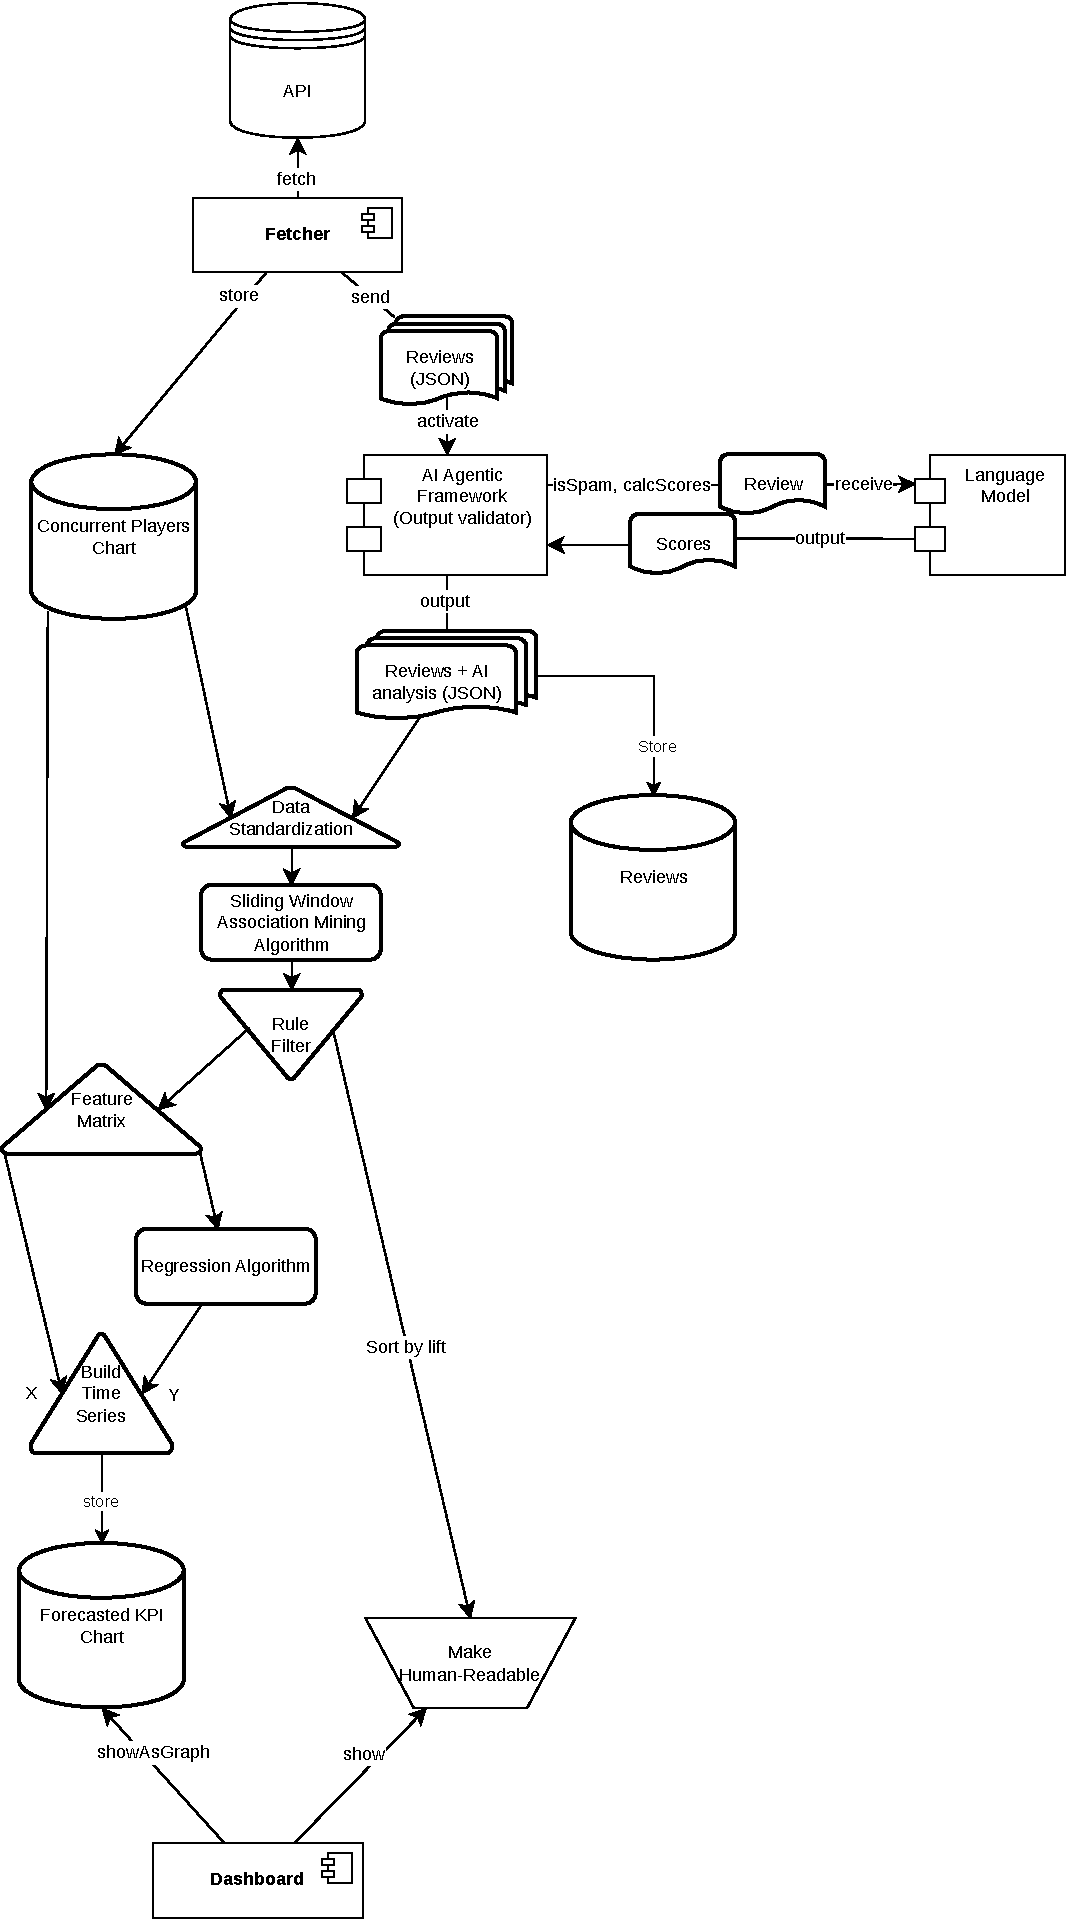
\includegraphics[width=0.8\linewidth]{figure/StARAPTORSystemArchitecture.pdf}
    \caption{The StARAPTOR pipeline. All stages read from and write to the per-game DuckDB database. An orchestrator (not shown) composes the stages into the initialization and daily pipelines and prevents concurrent runs; a local dashboard exposes forecasts, rules and reviews.}
    \label{fig:architecture}
\end{figure}

\subsection{Data Collection}
\label{sub:data_collection}

The \textbf{review stream} is retrieved from the Steam store review API, which exposes paginated batches of 100 reviews ordered from most to least recent. The fetcher walks the pagination cursor backwards one day at a time (a review is assigned to a day by its creation timestamp, and pagination for a day stops as soon as a batch crosses into the previous one): for each day it retains at most 250 reviews, composed of the top 125 reviews by \emph{weighted vote score}, the helpfulness score Steam assigns to each review, plus a uniform random sample of the remainder. This stratified design guarantees that the most informative reviews of each day are always analyzed, while the random component prevents the dataset from being biased towards already-popular reviews only. Duplicated reviews are filtered by identifier across days. For each review the system stores the identifier, the text, the language, the timestamps, the recommendation flag, the helpfulness (weighted vote) score, purchase-related flags (whether the game was purchased on Steam or received for free), the playtime at the moment the review was written, whether the reviewer primarily plays on Steam Deck, and, when available, hardware information (RAM, VRAM, GPU, CPU vendor, operating system, resolution) extracted from the review metadata.

The \textbf{KPI stream} consists of hourly concurrent-player observations retrieved from the games-popularity.com API\footnote{\url{https://games-popularity.com}}, which serves them newest-first and paginated through an opaque cursor; an optional API key, read from the \texttt{GAMES\_POPULARITY\_API\_KEY} environment variable, only raises the rate limits, while an unknown game (HTTP 404) simply yields no data. The hourly observations are aggregated into one row per day (mean, median, peak and minimum concurrent players). From the daily percentage change of the peak, each day is assigned a trend label used as a mining item (\texttt{kpi\_retention\_growth}, \texttt{kpi\_retention\_drop}, \texttt{kpi\_retention\_stable}): growth if the change is at least $+5\%$, drop if it is at most $-5\%$, stable otherwise.

\subsection{LLM-based Review Processing}
\label{sec:review_processing}

Raw review text cannot be mined directly: association rule mining operates on categorical items, so every free-text review must first be converted into structured attributes. StARAPTOR delegates this conversion to a Large Language Model invoked through a structured-output framework (Instructor\footnote{\url{https://github.com/567-labs/instructor}}), which constrains the model to return a schema-validated JSON object; responses that fail validation are retried rather than silently accepted.

For each non-empty review, the model returns a spam flag (ASCII art, memes, copypasta and joke texts without real feedback are discarded from the pipeline), an optional score from 1 to 5 for each of 12 game aspects (multiplayer, immersion, community, replayability, story, monetization model, gameplay, controls, graphics, customization, audio, difficulty), and a set of boolean indicators: whether the review appears useful, whether it contains positive and negative aspects, whether it contains a bug description, and whether the text actually recommends the title. Aspect scores are extracted only when the aspect is explicitly discussed in the review, so unmentioned aspects contribute no signal. The recommendation indicator is deliberately decoupled from Steam's official recommendation status: the system prompt instructs the model to judge the review's underlying sentiment, decoding sarcasm and irony. The prompt also counteracts the positivity bias known to affect LLM-based scoring by explicitly anchoring the low end of the scale (1--2) to poor or problematic experiences.

The stage runs with temperature 0 and disabled reasoning for deterministic and cost-efficient extraction, and issues requests concurrently under a configurable rate limit. It is precisely this agnosticism that motivates RQ1: since the entire downstream pipeline consumes model-generated attributes, the dispersion of such attributes across models of different classes must be quantified before the rest of the system can be trusted (Section~\ref{sec:evaluation_methods}).

\subsection{Association Mining Pipeline}
\label{sec:mining_pipeline}

Each processed review is converted into a \emph{transaction}, i.e., a set of categorical item tags: the aspect scores (e.g., \texttt{gameplay\_4}), the boolean flags (e.g., \texttt{containsBugDescription\_True}), the playtime at review discretized into five buckets (refund zone below 2 hours, casual below 10, mid-core below 50, heavy below 200, hardcore above), the review language, the available hardware attributes, and the KPI trend label of the day the review was published (e.g., \texttt{kpi\_retention\_drop}). Transactions therefore mix player characteristics, reported experience and the concurrent-player trend, which is what allows mined rules to connect review content to KPI behavior.

Mining is not performed on the whole history at once: reviews are grouped into overlapping sliding windows (by default 14 days wide, shifted by 7 days at a time), and a separate mining run is performed on each window containing at least 500 reviews. This guarantees that each run is based on a statistically meaningful sample and that the evolution of rules over time can be observed.

Each mining run applies the FP-Growth algorithm \cite{han2000fpgrowth} through the mlxtend implementation\footnote{\url{https://github.com/rasbt/mlxtend}}, with the following default thresholds: minimum support 0.02, minimum confidence 0.5 and minimum lift 1.2. Raw FP-Growth output, however, is known to be rich in patterns that are statistically valid but semantically weak \cite{fernandez2022survey_arm_text}. The mining stage therefore applies a cascade of heuristic filters:
\begin{enumerate}
    \item \textbf{near-universal item removal}: items appearing in more than 95\% of the transactions of a window are dropped before mining, as they carry no discriminative signal;
    \item \textbf{tautology filtering}: rules whose antecedent and consequent are identical are removed;
    \item \textbf{trivial hardware rules}: rules composed only of hardware attributes on both sides are removed, as they describe the players' machines rather than the game;
    \item \textbf{permutation pruning}: rules spanning the same item pool are collapsed to the highest-lift permutation;
    \item \textbf{antecedent deduplication}: for each antecedent, only the highest-lift rule is kept;
    \item \textbf{sub/super-redundancy pruning}: a more specific rule ($A \wedge B \rightarrow C$) is removed unless its confidence exceeds that of the corresponding general rule ($A \rightarrow C$) by at least 0.05.
\end{enumerate}
The surviving rules, together with the mining parameters and the window metadata, are persisted in the storage layer and identified by a run identifier. The adequacy of this cascade is exactly what the empirical verification study of Section~\ref{sec:evaluation_methods} is designed to assess.

\subsection{KPI Forecasting}
\label{sec:forecasting}

The forecasting stage trains an XGBoost regressor \cite{chen2016xgboost} on a daily feature matrix assembled from three sources:
\begin{itemize}
    \item \textbf{KPI history}: lagged levels (1, 7 and 14 days), 7-day rolling mean and maximum (strictly shifted to avoid information leakage), the daily peak percentage change, and the current level;
    \item \textbf{calendar features}: day of the week (as an integer and encoded with sine/cosine), a weekend flag and its interactions with the lagged levels;
    \item \textbf{review-derived features}: for each day, the mean of each of the 12 aspect scores over that day's non-spam reviews, the positive-review ratio, the daily review count, and one feature per mined association rule carrying the rule's lift on that date.
\end{itemize}

The regression target is not the raw player count, but the \emph{log-ratio} between the next day's and the current day's mean concurrent players. Tree-based models cannot extrapolate beyond the range observed at training time, so a model trained on absolute levels would be structurally blind to any future peak higher than the historical ones; relative variations are far more repeatable patterns that generalize across scales.

The model is tuned with Optuna \cite{akiba2019optuna} over tiers indexed by dataset size, and re-tuned only when the stored parameters are detected as stale, trading off accuracy and computational cost. Training also employs a custom asymmetric objective that penalizes underestimation more heavily than overestimation (with penalty multiplier $\alpha = 5$): for capacity-planning purposes, predicting too few players (under-provisioning) is more damaging than predicting too many.

The 30-day forecast is produced recursively: the model predicts one log-ratio at a time, and the predicted level is fed back as the anchor for the next day. Since future review content is unknown, review-derived and rule-derived features progressively decay towards their historical baselines. Finally, because chained log-ratio predictions systematically underestimate the expected level (a consequence of Jensen's inequality), a horizon-proportional correction based on the training residual variance is applied, optionally multiplied by a configurable safety buffer.

The evaluation protocol that quantifies the contribution of review-derived features and mined rules to the forecast, the subject of RQ3, is described in Section~\ref{sec:evaluation_methods}.

\section{Research Methods}
\label{sec:evaluation_methods}

\subsection{LLM-based NLP Performance Benchmark}
\label{sub:nlp_benchmark}

As StARAPTOR is model-agnostic, a direct performance benchmark on the processed output would not measure the quality of the system, but only the intrinsic quality of whichever model is configured. Moreover, no annotated ground truth exists for aspect-level review scoring, so the accuracy of individual extractions cannot be established against a gold standard. The benchmark therefore targets the property the framework actually depends on: the \emph{consistency} of the extracted attributes across models. If models of different classes produce comparable outputs on the same reviews, the downstream pipeline is robust to the choice of the model, which is what RQ1 asks.

\paragraph{Experiment design.} The benchmark uses a single stratified sample of 500 reviews drawn from the \emph{raw} review stream fetched live from the Steam store review API, not from the stored history (already spam-filtered by the pipeline), mirroring the daily sampling mix actually consumed by the pipeline: half of the reviews are the top-ranked by weighted vote score and half are uniformly random, covering the observed language distribution. Drawing the sample from the raw, unfiltered stream is a hard requirement of the method, not a convenience: the spam flag is part of the extraction schema, and only unfiltered reviews (spam included) make inter-model differences in spam recognition measurable. The sample is frozen before execution and identified by a fixed sampling seed, so that the same review set can be re-used to benchmark future models. Each tested model processes the whole sample with identical prompts and, where possible, identical decoding configuration (\texttt{temperature}, \texttt{top\_p} and \texttt{top\_k}), so that the model is the only variable of the experiment. The tested models, grouped into performance classes by parameter count, are listed in Table~\ref{tab:model_configurations}.

\begin{table}[H]
    \centering
    \caption{Tested models and shared configuration of the RQ1 benchmark.}
    \label{tab:model_configurations}
    \vspace{1mm} % Adjust the height of the space between caption and tabular
    \begin{tabular}{>{\raggedright\arraybackslash}p{0.11\linewidth} >{\raggedright\arraybackslash}p{0.39\linewidth} >{\centering\arraybackslash}p{0.12\linewidth} >{\centering\arraybackslash}p{0.22\linewidth}}
        \toprule
        \rowcolor{black}
        \textbf{\textcolor{white}{Class}} & \textbf{\textcolor{white}{Model}} & \textbf{\textcolor{white}{Params}} & \textbf{\textcolor{white}{Quantization}}\\
        \midrule
        \multirow{2}{*}{Large} & \texttt{Muse-Glimmer-30B} & 30B & UD-Q4\_K\_XL\\
        \cmidrule{2-4}
         & \texttt{Qwen3.8-27B} & 27B & UD-Q4\_K\_XL\\
        \cmidrule{1-4}
        Medium & \texttt{gemma-4-12B-it} & 12B & UD-Q8\_K\_XL\\
        \cmidrule{1-4}
        Small & \texttt{gemma-4-E4B-it} & E4B & UD-Q8\_K\_XL\\
        \midrule
        \multicolumn{4}{@{}p{0.86\linewidth}@{}}{\textbf{Configuration details:} temperature $0.0$ (\texttt{top\_p}/\texttt{top\_k} left at server defaults); thinking disabled (\texttt{enable\_thinking=false}), reasoning budget $0$.

        \textbf{Performance classes} by parameter count: Large $\geq$ 20B, Medium 10--20B, Small $<$ 10B. Models quantized dynamically by Unsloth\footnote{hf.co/unsloth}.}\\
        \bottomrule
    \end{tabular}
\end{table}

\paragraph{Reliability metrics.} For each review and aspect, the outputs of the different models are compared through Krippendorff's alpha \cite{krippendorff2004}, a chance-corrected inter-rater reliability coefficient that supports multiple raters and ordinal measurement. Since an aspect a model does not score is, by design, a prediction of absence (encoded as 0 on the same 0--5 scale consumed by the downstream stages), every model produces a complete rating for every review-aspect pair: the primary coefficient is therefore the ordinal alpha computed on the full 0--5 scale, which measures agreement on exactly the signal the pipeline consumes, absences included. The chance correction is essential in this setting: most review-aspect pairs are zeros, and raw agreement would be inflated by trivial concordances.

Because the scale mixes two distinct judgments, reliability is also decomposed into two components: detection agreement (absence versus presence, computed with the nominal variant of the coefficient) and rating agreement (the ordinal variant restricted to the aspects that all models detect). The decomposition shows whether a loss of reliability originates in models seeing different aspects or in models scoring the same aspects differently. In addition, because the sample is drawn from the raw stream, the binary spam flag is benchmarked as a further rated attribute: the nominal alpha over the models' spam decisions, with its bootstrap confidence interval and the number of reviews a majority flags as spam, measures the inter-model reliability of spam recognition itself. Each estimate is reported per aspect together with the number of units it is based on, and confidence intervals are obtained by bootstrapping over the sampled reviews; aspects whose jointly detected ratings are too few for a stable estimate are explicitly reported as insufficient data. Following Krippendorff's interpretation, $\alpha \geq 0.800$ is treated as reliable agreement and $\alpha \geq 0.667$ as the lowest limit for tentative conclusions: these thresholds operationalize RQ1.

\paragraph{Aggregate-level dispersion.} To connect the benchmark to the actual use of the extracted attributes, a second dispersion measure is computed at the aggregate level: the daily per-aspect means and the daily positive-review ratio, which are the exact features consumed by the forecasting pipeline (Section~\ref{sec:forecasting}), are derived once per model and compared across models through their relative dispersion. Low dispersion at both the review level and the aggregate level indicates that the framework is robust to the choice of the underlying model. Consistency, however, does not imply correctness: models sharing a systematic bias would agree while being jointly wrong; this threat is mitigated by the anti-bias anchoring of the extraction prompt (Section~\ref{sec:review_processing}). The results of this benchmark are reported in Chapter~\ref{chap:results} and used to answer RQ1.

\paragraph{From benchmark to production labels.} The benchmark does more than measure consistency: the model whose extractions agree most with the cross-model majority on every field (the consensus criterion, i.e., the highest majority-agreement score) is selected as the base model of the study. Its extractions over the frozen sample are stored in the review database, and the same model then re-processes the whole fetched review pool, upserting the results into the same table, so that the downstream stages (RQ2 and RQ3) operate on a single consistent labeling of the entire review history.

\subsection{Empirical Verification of Mined Rules}
\label{subsec:rules_verification}

As detailed in Section \ref{sec:mining_pipeline}, the mining stage of StARAPTOR does not return the raw output of FP-Growth: every mining run passes through a cascade of heuristic filters (removal of near-universal items, minimum support, confidence and lift thresholds, tautology filtering, removal of purely hardware-based rules, and permutation and redundancy pruning) designed to discard patterns that are statistically valid but semantically uninformative.

These filters, however, are \emph{objective} interestingness criteria: they encode assumptions about the statistical soundness of a rule (as its frequency, its predictive confidence and its non-redundancy) but they cannot establish whether a rule is meaningful to a developer. The distinction between objective and subjective (i.e., actionable and unexpected) interestingness is well established in the association mining literature \cite{eldin2026interestingness}: a rule with high lift may still be a spurious artifact of the item taxonomy rather than a genuine pattern in the underlying reviews. For this reason, the mined rule sets cannot be taken at face value, and the empirical study described in this section was designed to answer two complementary questions:

\begin{enumerate}
    \item \textbf{Filter adequacy}: did any statistically valid but semantically uninformative rule survive the filtering cascade?
    \item \textbf{Rule utility}: are the surviving rules actionable, i.e., grounded in actual review content and interpretable as insight a developer could act upon?
\end{enumerate}

\paragraph{Choice of the evaluation method.} No ground truth exists for this task: there is no labeled corpus of ``valid'' associations between review patterns and player behavior against which the mined rules could be automatically compared. Constructing such an oracle would require manually annotating the very associations the system is meant to discover, making the evaluation circular and confining it to the specific games and periods inspected. Downstream quantitative evidence cannot serve this purpose alone either: a rule set may improve the forecasting regressor by exploiting spurious correlations that carry no interpretable information. Therefore, in line with common practice in exploratory association rule mining studies \cite{fernandez2022survey_arm_text}, the mined rules were evaluated through systematic inspection governed by an explicit protocol. To make the evaluation reproducible, the protocol operationalizes the subjective interestingness dimension with a deterministic, rule-based classifier whose thresholds are derived from the data itself, rather than with free-form manual judgment; a manual annotation pass remains available as an optional validation layer, and its agreement with the rule-based labels is reported alongside the results.

\paragraph{Inspection protocol.} The inspection followed a protocol that was fixed before examining any rule set, and consisted of three stages.

\emph{Sampling.} For each game in the study and each historical mining window, the top 10 rules by lift were selected, together with 5 rules drawn uniformly at random from the remainder of the window's rule set (using a fixed random seed, reported in Section \ref{sec:mining_results}). The former represent the rules the system would surface first in practice; the latter ensure that the evaluation is not limited to the most prominent rules. Sampled rules were exported in shuffled order, so that prominence could not be inferred from the presentation.

\emph{Classification rubric.} Each sampled rule was assigned to exactly one of four mutually exclusive categories, operationalized on the item taxonomy of Section \ref{sec:mining_pipeline}: (i)~\emph{actionable}, if the rule links semantic review content (aspect scores, bug-related flags, playtime buckets) to a semantically rich pattern on which a developer could act; (ii)~\emph{semantically trivial}, if the consequent is entailed by the antecedent or by the label definitions, so that the rule merely restates the overall polarity of the review or the definitions of the extracted flags; (iii)~\emph{taxonomy artifact}, if the association is mediated by the structure of the items rather than by the domain, e.g., by language, hardware, purchase or KPI-state attributes; (iv)~\emph{unclear}, if the association is near statistical independence and carries no interpretable signal.

Classification is performed by a fixed decision procedure, applied in order with first match winning, summarized in Table~\ref{tab:classification_rules}. The procedure distinguishes structural items (prefixes \texttt{lang\_}, \texttt{hw\_}, \texttt{playtime\_}, \texttt{kpi\_}, \texttt{steam\_purchase}, \texttt{received\_for\_free}) from content items (the 12 aspect scores and the bug flag), and derives two parameters directly from the stored non-spam reviews of the game under study: the base rate of every item, and the entailment relation between label items, defined as a measured conditional probability of at least 0.90. Entailment is deliberately asymmetric: e.g., \texttt{voted\_up\_True} entails \texttt{actuallyRecommendsTitle\_True} with probability 0.942, whereas the reverse direction holds only with probability 0.57 (many non-recommending reviews are still positive overall), so only the former is treated as entailed. A rule whose consequent also carries content items is never demoted by the entailment check: it is judged on its content by the remaining rules.

\begin{table}[H]
    \centering
    \caption{The fixed decision procedure of the rule-based inspection protocol. Rules are evaluated in order; the first matching rule assigns the category.}
    \label{tab:classification_rules}
    \begin{tabular}{>{\centering\arraybackslash}p{0.07\linewidth} >{\raggedright\arraybackslash}p{0.64\linewidth} >{\raggedright\arraybackslash}p{0.15\linewidth}}
        \toprule
        \rowcolor{black}
        \textbf{\textcolor{white}{Rule}} & \textbf{\textcolor{white}{Condition}} & \textbf{\textcolor{white}{Category}}\\
        \midrule
        R1 & consequent items are a subset of the antecedent items & semantically trivial\\
        R2 & a consequent item is entailed by an antecedent label item (measured conditional $\geq 0.90$) and the remaining consequent items are structural, near-universal (base rate $\geq 0.90$) or already in the antecedent & semantically trivial\\
        R3 & every item of the rule is structural & taxonomy artifact\\
        R4 & the antecedent consists only of demographic items (\texttt{lang\_}, \texttt{hw\_}, \texttt{playtime\_}) & taxonomy artifact\\
        R4b & the consequent consists only of structural items & taxonomy artifact\\
        R5 & every consequent item has base rate $\geq 0.90$ (base-rate restatement) & semantically trivial\\
        R6 & lift $< 1.5$ (near independence) & unclear\\
        R7 & none of the above & actionable\\
        \bottomrule
    \end{tabular}
\end{table}

\emph{Trace-back verification.} Every rule classified as actionable was traced back to its supporting reviews: a sample of up to 10 stored reviews whose transaction contains the antecedent items was retrieved from the database, to confirm that the association reflects actual review content rather than an artifact of the discretization.

\emph{Redundancy.} Independently of the categories, rule redundancy was measured automatically: a sampled rule is redundant if its full item-set signature (sorted antecedents plus consequents) appears in more than one sampled rule, i.e., near-duplicates surviving the miner's pruning.

The outcome of each inspection was recorded in a structured form (rule identifier, window, category, and supporting evidence), from which the residual noise rate and the actionability rate reported in Chapter~\ref{chap:results} were computed. A manual annotation pass is optional: when a human-annotated form is provided, the agreement between the rule-based and the human labels is reported as a validation metric.

\paragraph{Cross-window persistence.} To complement the qualitative analysis with a quantitative signal, the historical mining runs were also compared across sliding windows: an association that re-occurs across independent windows is less likely to be a spurious artifact of a single period, and is therefore used as a proxy for the robustness of the mined patterns.

The quality metrics associated with this study are the \emph{residual noise rate} (the fraction of inspected rules that should have been filtered out), the \emph{actionability rate} (the fraction of inspected rules deemed actionable), the \emph{persistence rate} (the fraction of rules re-occurring across independent windows), and the \emph{redundancy rate} (the fraction of sampled rules whose full item-set signature is duplicated). Together, these metrics provide the evidence used to answer RQ2 in Chapter~\ref{chap:results}.

\subsection{Forecasting Evaluation}
\label{sub:forecasting_evaluation}

The contribution of review-derived features and mined associations to the forecast is quantified through an ablation study on the regressor: the forecasting pipeline is trained and evaluated three times, with a progressively richer feature set and everything else held constant. The three configurations are:
\begin{itemize}
    \item \textbf{C1 (baseline)}: KPI history and calendar features only, reproducing a KPI-only forecasting system within the same framework;
    \item \textbf{C2 (reviews)}: C1 plus the daily review aggregates (per-aspect means, positive-review ratio, daily review count);
    \item \textbf{C3 (full system)}: C2 plus the association rule features mined by the pipeline.
\end{itemize}
The comparison is internally fair by construction: the baseline is not an external system but the same pipeline deprived of the review-derived features, so any performance difference is attributable to the features alone rather than to implementation differences. A positive answer to RQ3 corresponds to a monotonic improvement from C1 to C2 to C3, with the gap between C1 and C3 measuring the overall improvement over a KPI-only forecaster.

\paragraph{Experiment design.} All configurations share the same regressor (XGBoost), the same asymmetric objective and the same recursive forecasting procedure, and each configuration undergoes an independent Optuna tuning pass: reusing the hyperparameters tuned for one feature set on the others would bias the comparison, since different feature sets may favor different parameter settings. Evaluation uses a chronological 70/30 split: the model is trained on the first 70\% of the available days and evaluated on the remaining 30\%, never used for training or tuning, so that temporal order is preserved throughout. Where more than one game is studied, the whole procedure is repeated independently per game.

\paragraph{Evaluation metrics.} Forecast quality is measured with MAE, RMSE and MAPE, reported both for the one-day-ahead prediction and for the recursive 30-day forecast, the latter being the quantity the system actually delivers. Since concurrent-player counts exhibit weekly seasonality, the metrics are additionally broken down by weekday and weekend days, and the underestimation rate is reported in accordance with the capacity-oriented objective. The improvement of C2 and C3 is expressed as relative error reduction with respect to the C1 baseline.

\paragraph{Feature importance analysis.} To complement the aggregate comparison, the trained C3 model is inspected through its gain-based feature importance, i.e., the total loss improvement attributed to the splits made on each feature during training. Two quantities are reported: the share of the total gain absorbed by the rule features, which shows whether the regressor actually exploits the mined associations rather than ignoring them, and the ranking of the highest-gain rules, which identifies which specific associations carry forecasting value. This analysis introduces no additional training, as the importance scores are a by-product of the model already trained for C3.

\paragraph{Interpretation safeguards.} An ablation study shows that a feature group contributes to the forecast, not why it contributes; likewise, gain importance is descriptive rather than causal evidence, as it shows that the regressor leans on a feature, not that the feature drives player counts. An improvement in C3 could in principle be driven by spurious rules; the outcome of C3 is therefore read jointly with the RQ2 study, and is strengthened when the rules with the highest gain are also among those classified as actionable by the inspection study. These results are reported in Chapter~\ref{chap:results} and used to answer RQ3.
